\documentclass[12pt]{article}
\usepackage{a4wide}
\usepackage{color, amssymb}
\usepackage[margin=1in]{geometry}
\usepackage[document]{ragged2e}
\usepackage[table]{xcolor}
\usepackage{multirow}
\usepackage[braket, qm]{qcircuit}
\setlength{\arrayrulewidth}{0.5mm}
\setlength{\tabcolsep}{16pt}
\renewcommand{\arraystretch}{1.9}
\usepackage[english,greek]{babel}
\usepackage{braket}
\usepackage{mathtools}
\usepackage{ragged2e}
\renewcommand{\baselinestretch}{1.5}
\input{epsf}
\usepackage{float}
\usepackage{graphicx}
\usepackage{caption}
\usepackage{subcaption}
\usepackage{cancel}
\usepackage{algorithm}
\usepackage[noend]{algpseudocode}

\begin{document}

\greektext

\noindent\rule{\textwidth}{2pt}
\begin{center}
{\bf ΥΠΟΛΟΓΙΣΤΙΚΗ ΓΕΩΜΕΤΡΙΑ}\\ 
{\bf 3o Σετ Ασκήσεων }\\
{\bf Καλαμαράκης Θεόδωρος:} 2018030022\\
\end{center}
\rule{\textwidth}{.5pt}
\noindent

\begin{center}

\end{center}
 
 

\justifying

\section*{Άσκηση 1}
    Για την υλοποίηση θα χρησιμοποιήσουμε \textlatin{priority search tree} και το πρόβλημα θα λυθεί ως μια παραλλαγή του προβλήματος αναζήτησης τριών πλευρών. Η συνθήκη για να τέμνονται δύο ορθογώνια με συντεταγμένες $(a_1,b_1,a_2,b_2)$ και $(x_1,y_1,x_2,y_2)$ 
    (οπου $(a_1,b_1),(x_1,y_1)$ οι κάτω αριστερά κορυφές και $(a_2,b_2),(x_2,y_2)$ οι πάνω δεξιά ), ειναι η:
    $$\left(b_1\leq y_2 \land b_2 \geq y_1\right) \land \left(a_1\leq x_2 \land a_2 \geq x_1\right)$$
    \begin{figure}[H]
        \centering
        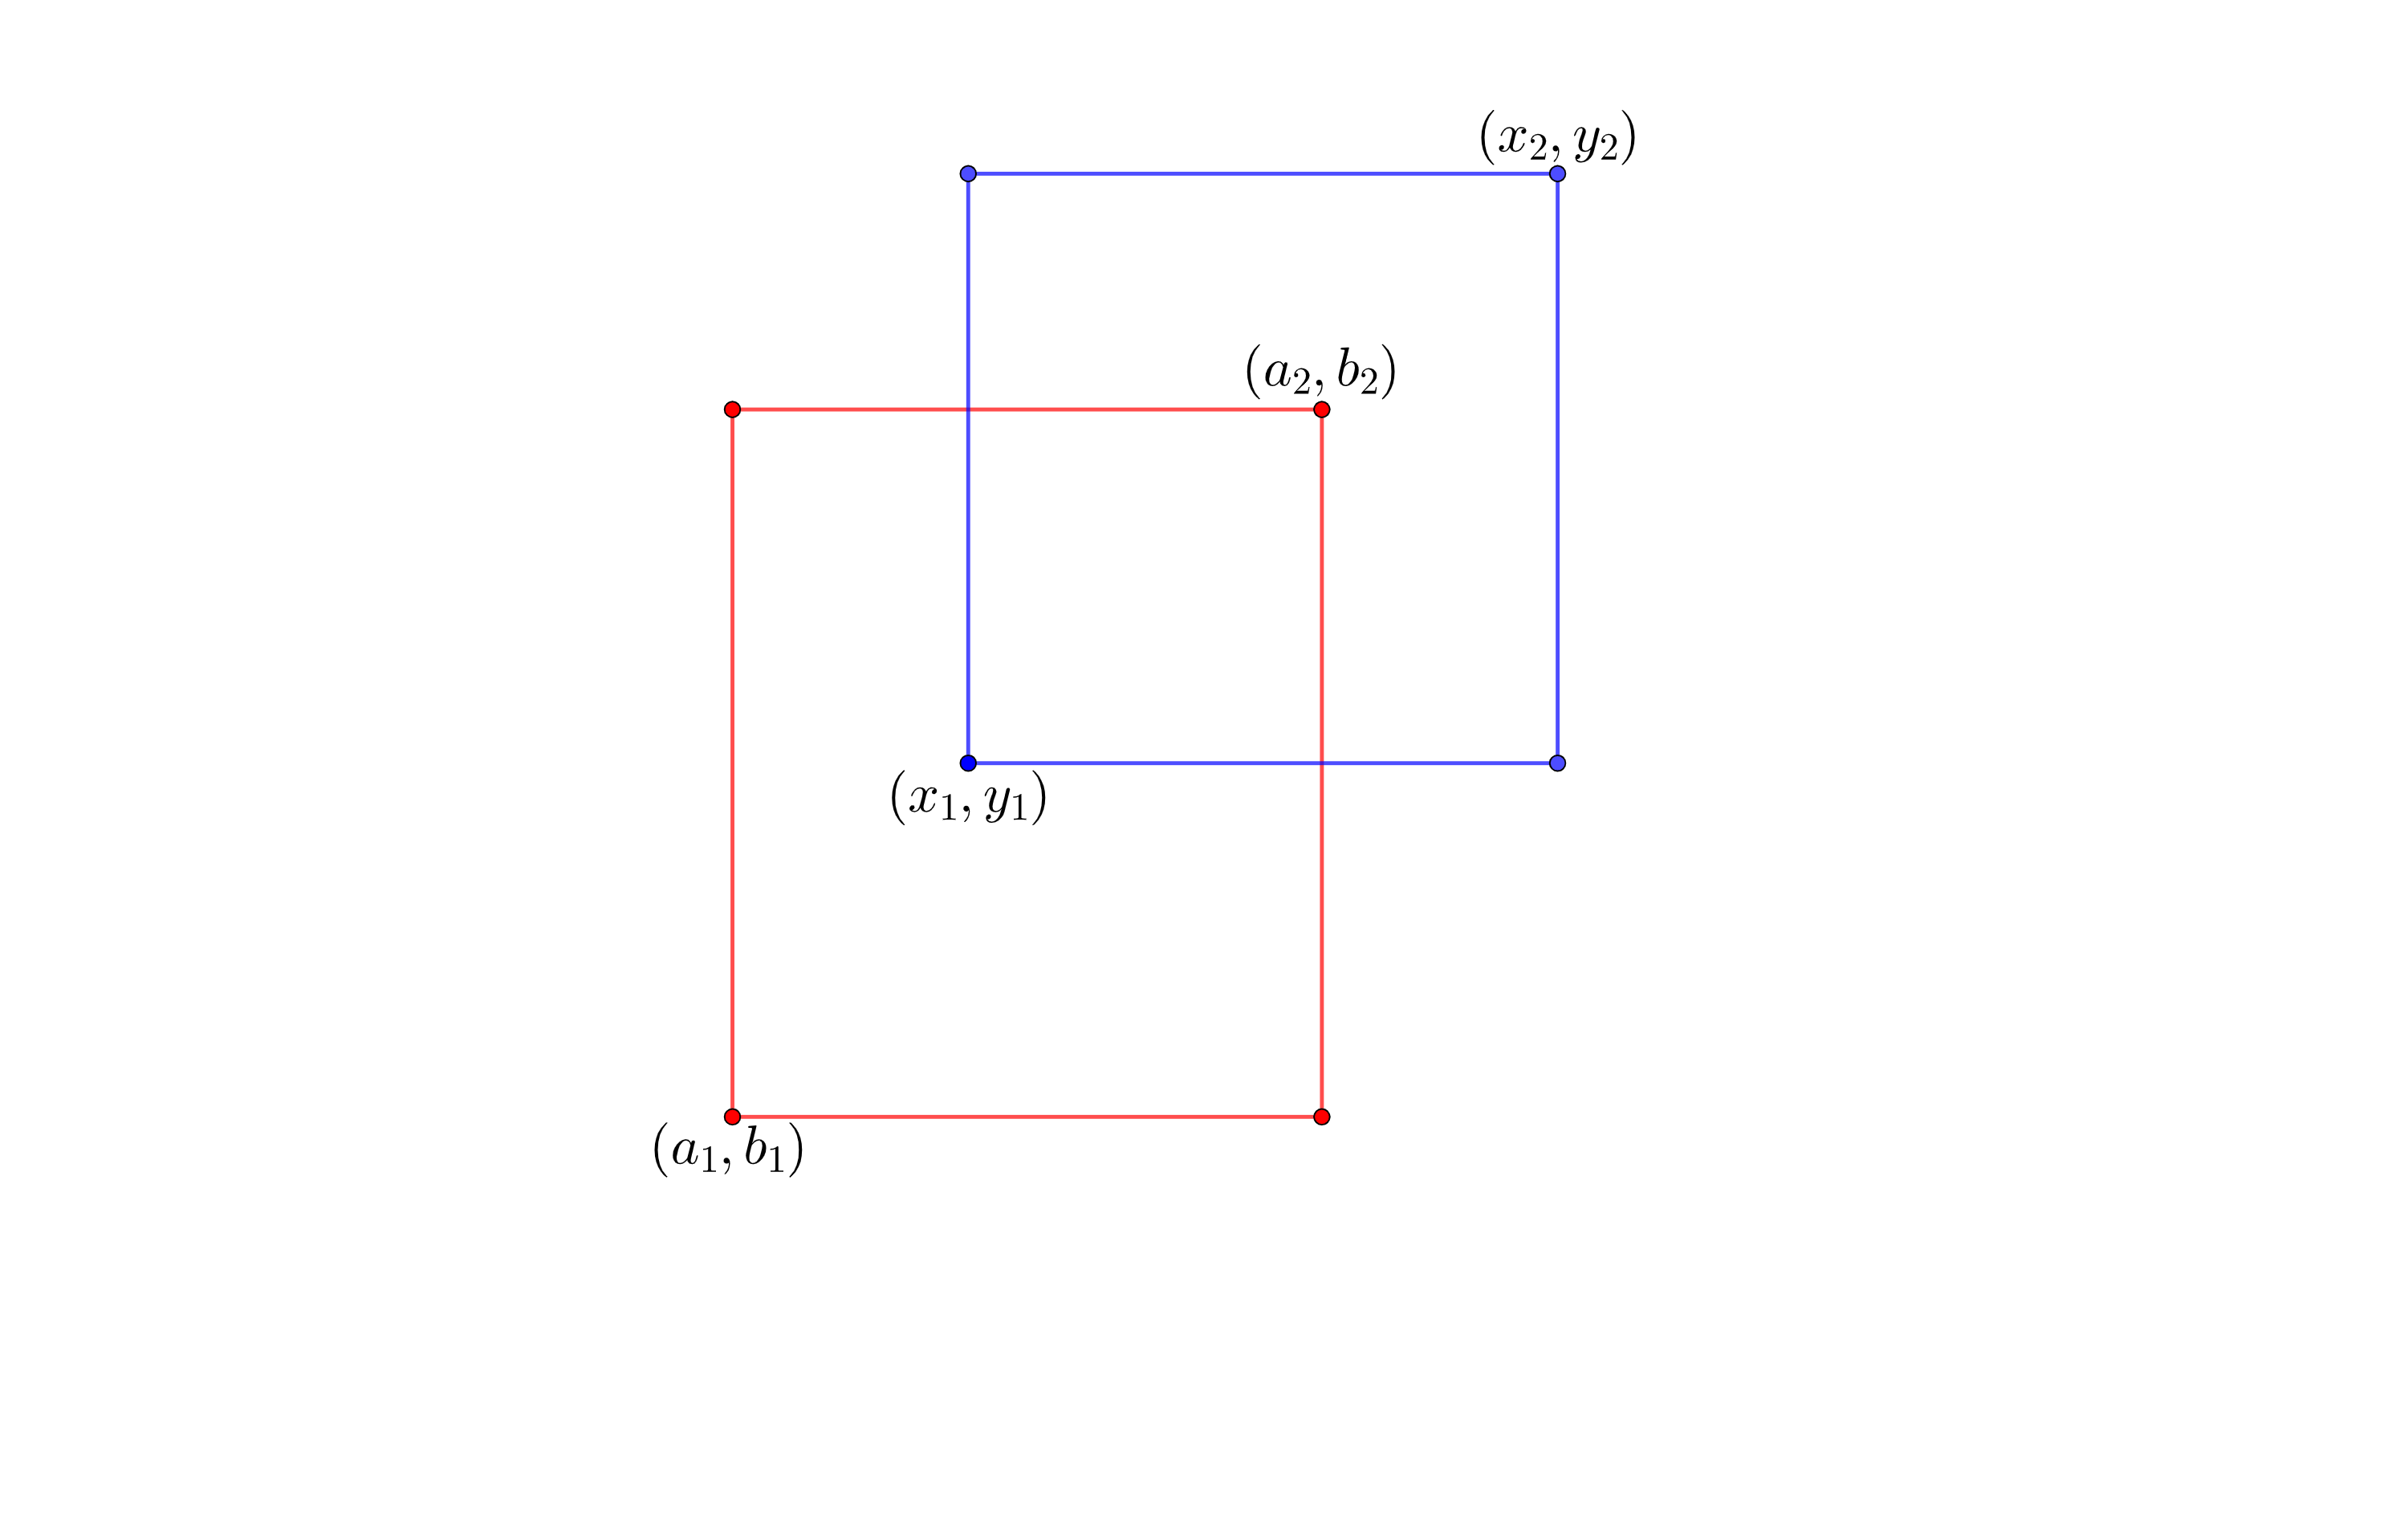
\includegraphics[scale = 0.7]{geogebra-export.png}
        \caption*{Σχήμα 1}
    \end{figure}

    Θα προσεγγίσουμε το πρόβλημα χρησιμοποιώντας την δομή \textlatin{priority search tree} με τον εξής τρόπο:\\
    Έχουμε ένα σύνολο $S$ με $n$ \textlatin{rectangles} $(x_1,y_1,x_2,y_2)$ τα οποία τοποθετούμε στο \textlatin{priority search tree} αλλά στην πράξη το κάθε \textlatin{rectangle} θα αντιπροσωπεύεται μόνο απο το πάνω δεξιά σημείο του $(x_2,y_2)$ δηλαδή θα είναι σαν να εφαρμόζουμε \textlatin{priority search tree} στα σημεία  $(x_2,y_2)$.
    (θυμίζουμε οτι ενα \textlatin{rectangle} το ορίζουμε χρησιμοποιώντας την κάτω αριστερα κορυφη του $(x_1,y_1)$ και τη πάνω δεξια $(x_2,y_2)$ )
    \begin{itemize}
        \item Κάθε κόμβος έχει 2 κλειδιά, $x_{2p} \in \mathbb{R}$ και $q \in U$.
        \item $x_{2p} =$ η \textlatin{median} $x_2$-συντεταγμένη
        \item $q =(x_1,y_1,x_2,y_2) \in U$ το σημείο με τη μεγαλύτερη $y_2$-συντεταγμένη
        \item Χωρίζουμε το $U - q$ ως προς το $x_{2p}$ και φτιάχνουμε αναδρομικά τα υποδέντρα.
        \item \textlatin{binary search tree} ως προς $x_2$
        και \textlatin{priority heap} ώς προς $y_2$ 
    \end{itemize}
     Η κατασκευή του δέντρου εχει κόστος $O(n\log n)$.

    Έστω οτι θέλουμε να αναζητήσουμε τις τομές ενός \textlatin{rectangle} απο το $S$ με συντεταγμένες $(a_1,b_1,a_2,b_2)$. 
    \begin{itemize}
        \item Αφαιρούμε απο το δέντρο τον κόμβο που\\ αντιστοιχεί στο   \textlatin{rectangle} $(a_1,b_1,a_2,b_2)\;\;\;\rightarrow \;\;O(\log n)$
        \item Κάνουμε αναζήτηση τριών πλευρών στο \textlatin{query} $[a_1,a_2]\times [b_1, +\infty ]$ όπως φαίνεται στο σχήμα. $\;\;\;\rightarrow \;\;O(\log n +k)$
        \begin{figure}[H]
            \centering
            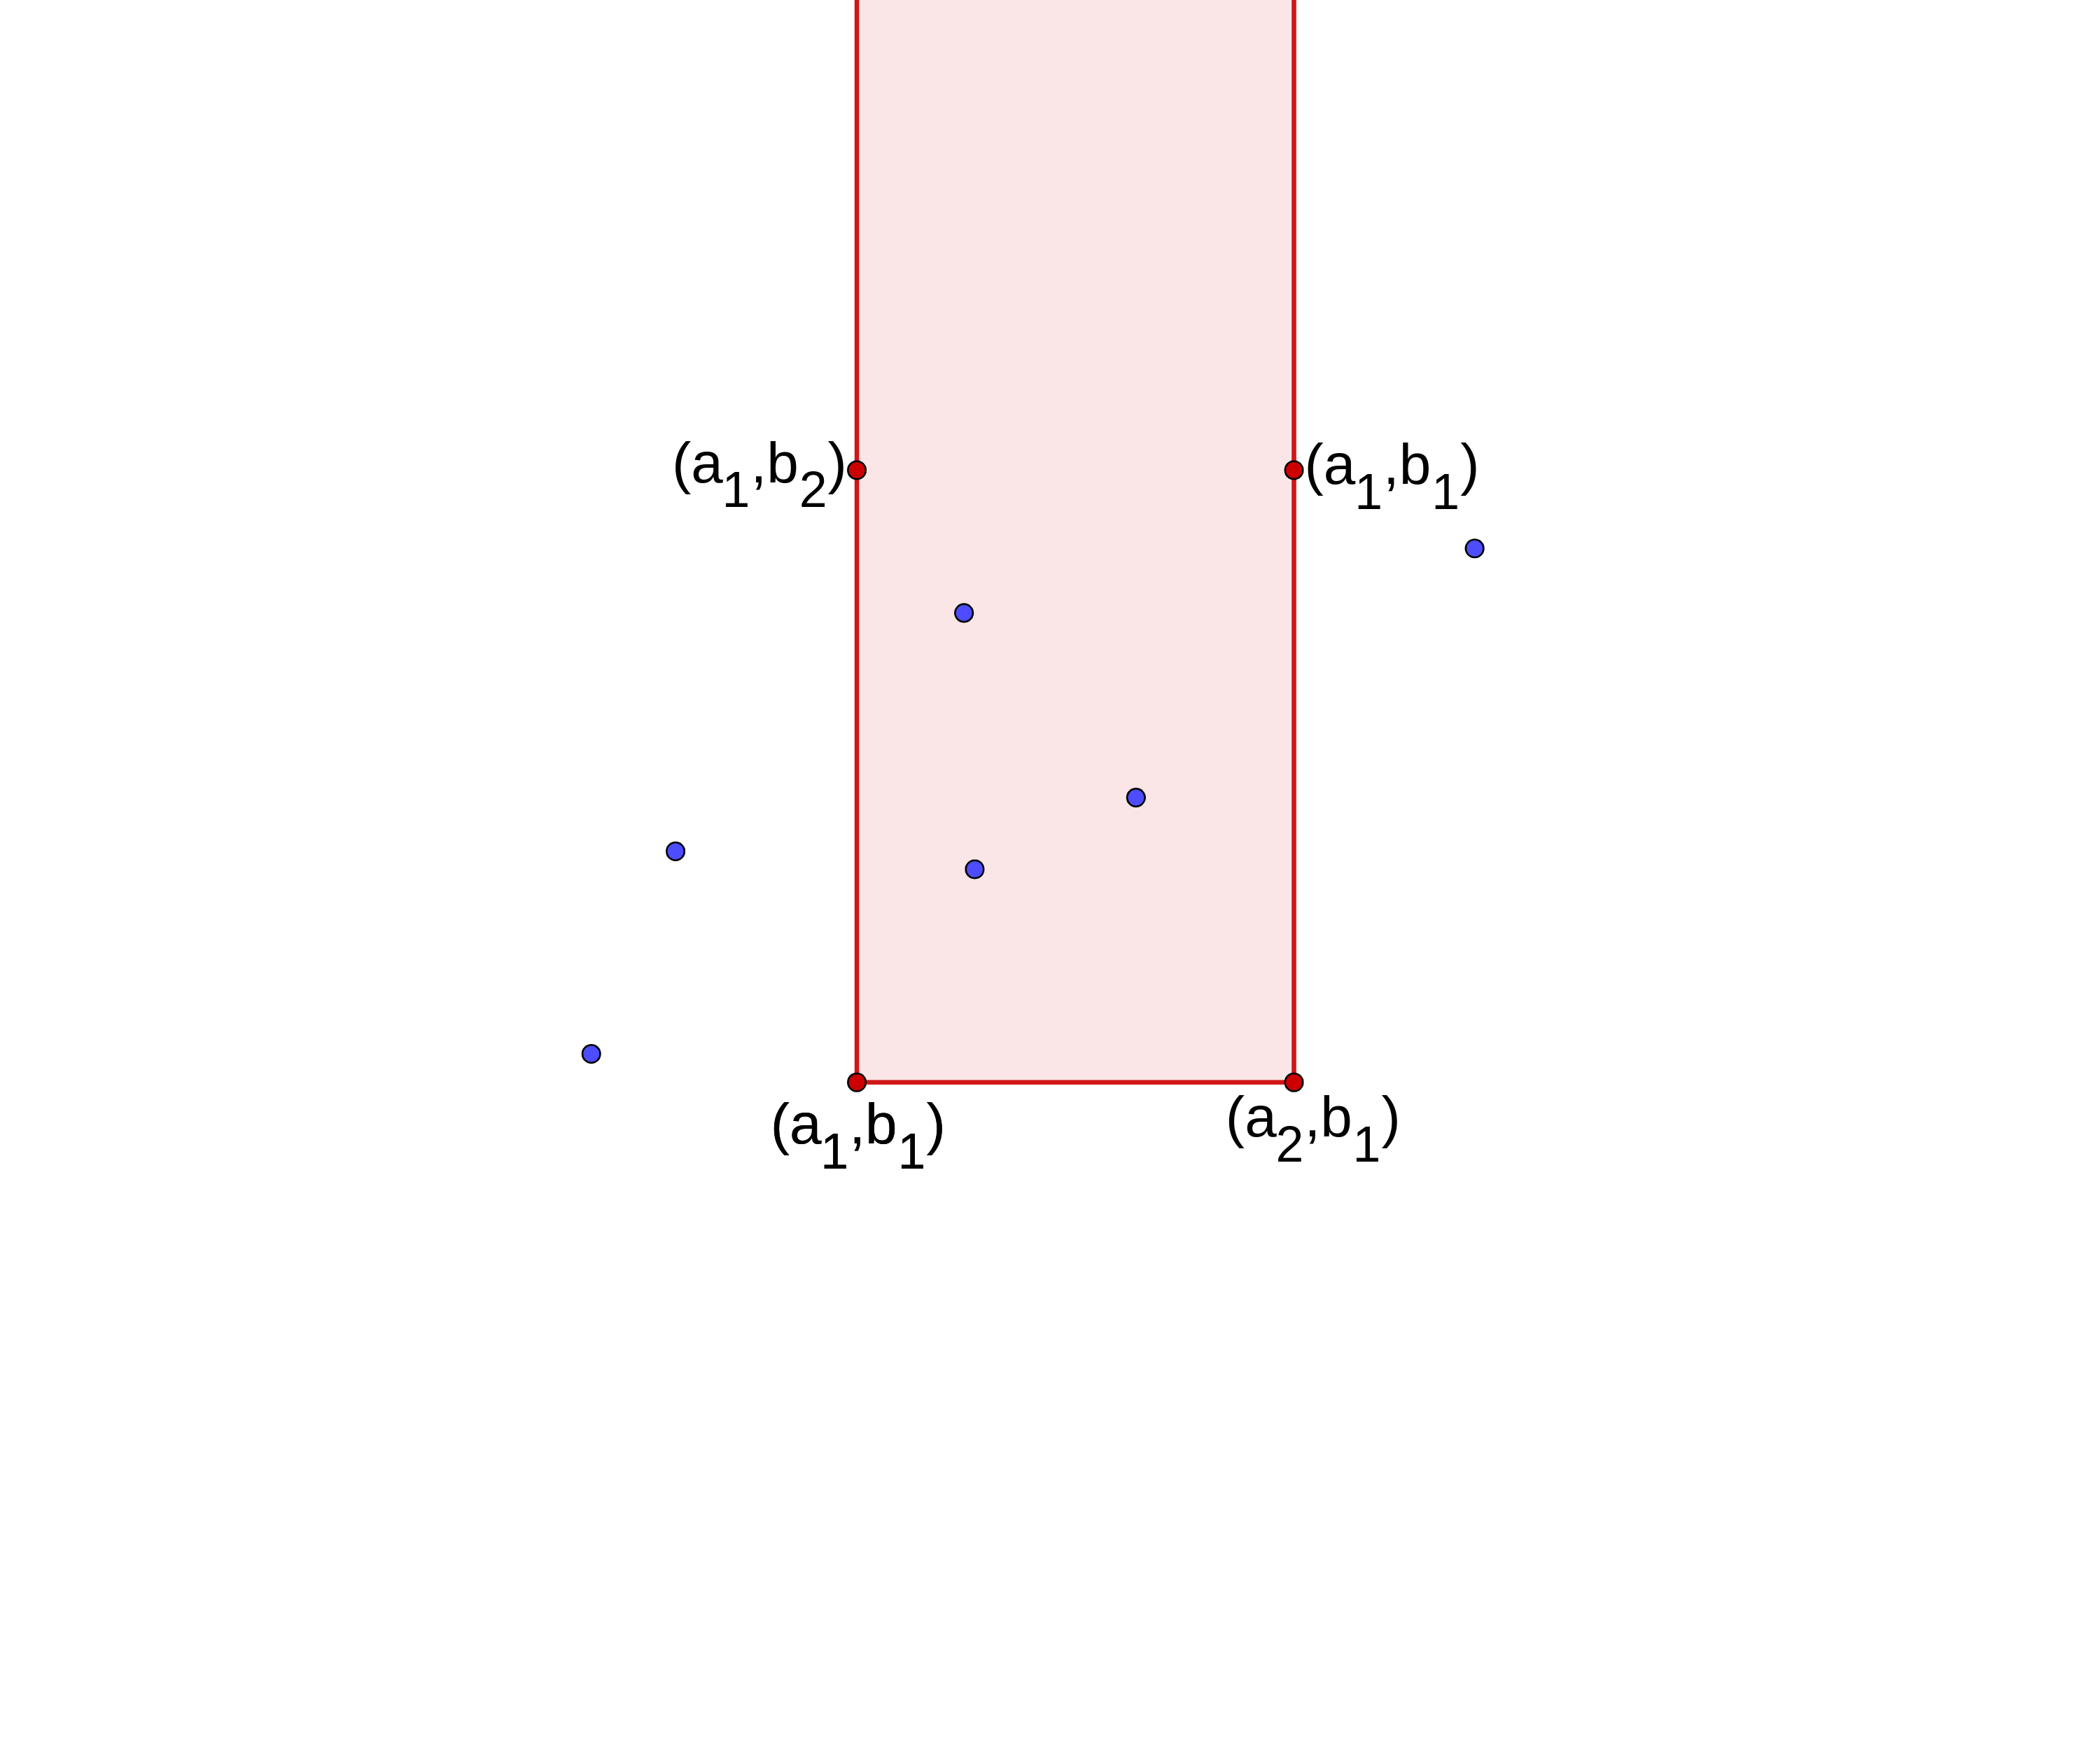
\includegraphics[scale = 0.4]{geogebra-export3.png}
            \caption*{Σχήμα 2}
        \end{figure}
        \item Σε αντίθεση με την απλή αναζήτηση τριών πλευρών, για κάθε σημείο $q$ που εντοπίζουμε να βρίσκεται εντός των τριών πλευρών, πρίν το κάνουμε \textlatin{report}, θα απαιτήσουμε επιπλέον να ισχύει $q.y_1\leq b_2$ 
        \item Μόλις ολοκληρωθεί η αναζήτηση τριών πλευρών θα ξαναεισάγουμε το \textlatin{rectangle} $(a_1,b_1,a_2,b_2)$  στο δέντρο $\;\;\;\rightarrow \;\;O(\log n)$
    \end{itemize}

    Με την παραπάνω αναζήτηση επιτυγχάνουμε να εντοπίσουμε όλα τα \textlatin{rectangles} $(x_1,y_1,x_2,y_2)$ τα οποία τέμνουνε απο αριστερά το $(a_1,b_1,a_2,b_2)$, είτε περικλείονται μέσα σε αυτο.
    (δηλαδή $a_1\leq x_2 \leq a_2 \land \left(b_1\leq y_2 \land b_2 \geq y_1\right)$). Τέτοια \textlatin{rectangles} είναι τα πράσινα του παρακάτω σχήματος.
    \begin{figure}[H]
        \centering
        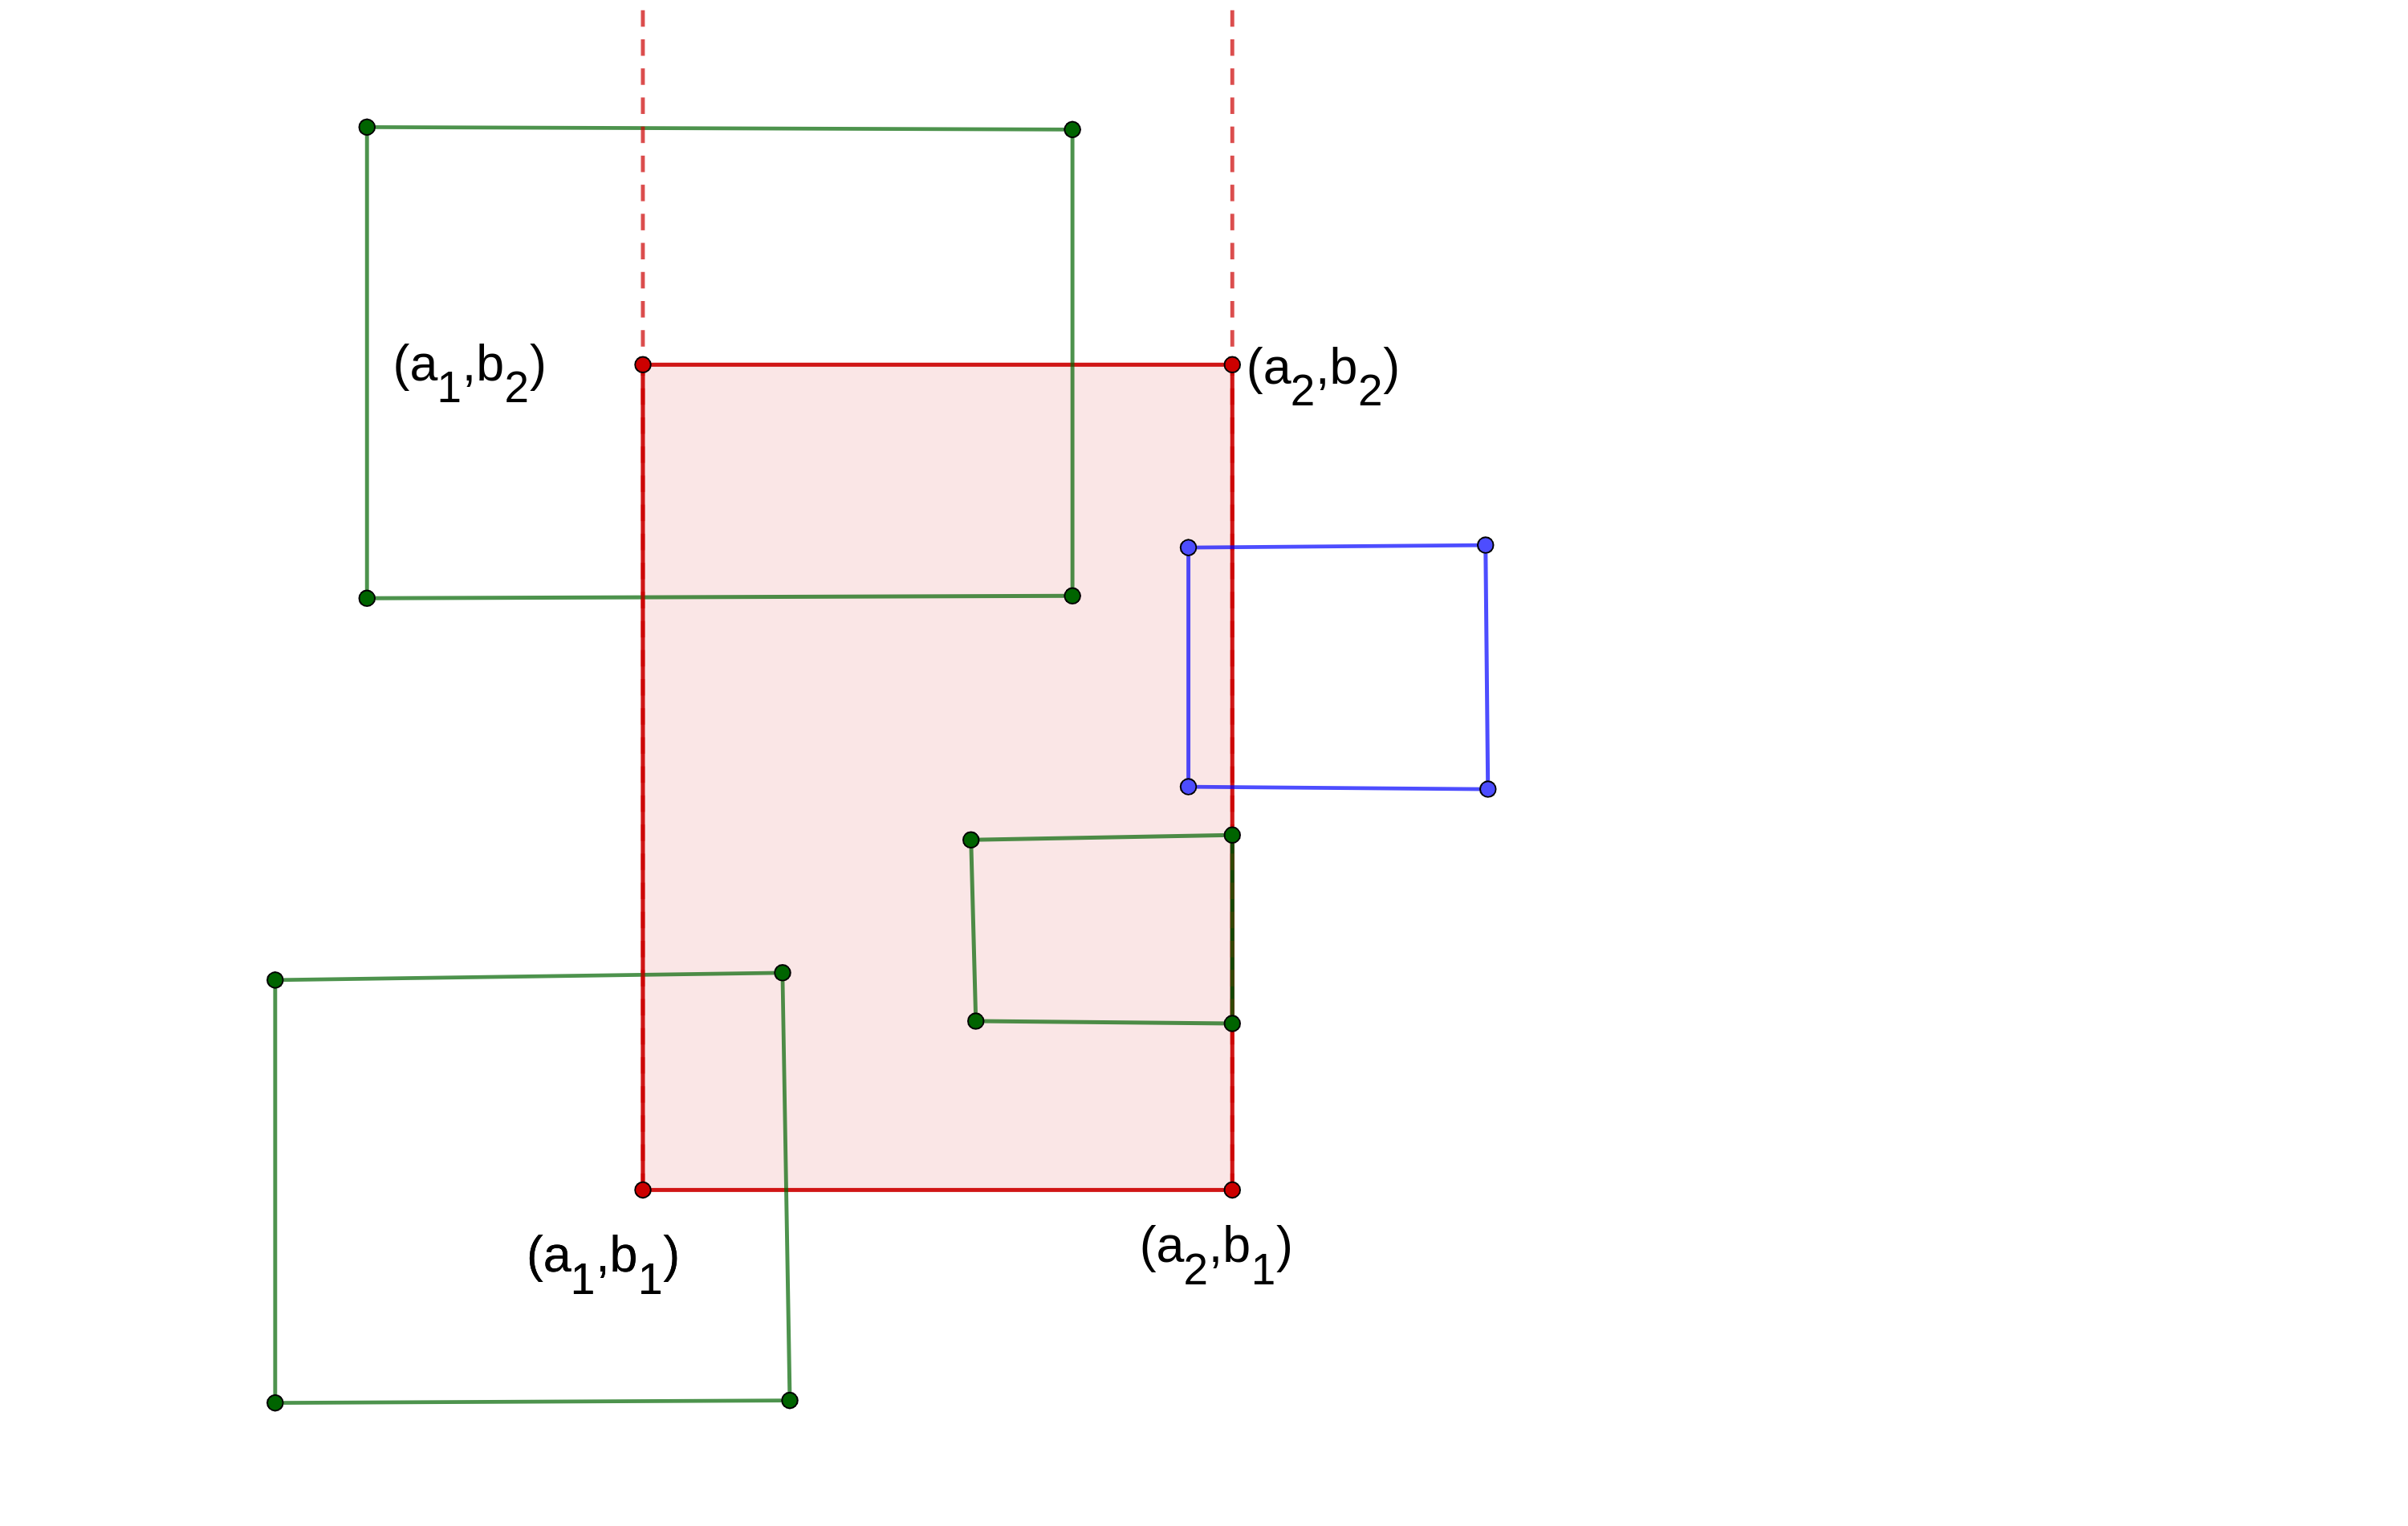
\includegraphics[scale = 0.6]{geogebra-export5.png}
        \caption*{Σχήμα 3}
    \end{figure}
    Το κόστος της αναζήτησης των αριστερών τομών για το \textlatin{rectangle} $i = (a_1,b_1,a_2,b_2)$ είναι 
    $$Q_i(n) = O(\log n) +O(\log n) + O(\log n + k_i) = O(\log n + k_i)$$
    όπου $k_i$ το πλήθος τών τομών. Η αναζήτηση αυτή θα επαναληφθέι για όλα τα \textlatin{rectangles} του $S$, οπότε οι τομές σαν αυτη του κόκκινου με το μπλέ στο Σχήμα 3 θα εντοπιστούν
    όταν γίνει αναζήτηση τρίων πλευρών με βάση το μπλέ \textlatin{rectangle} (θα γίνει \textlatin{report} η τομή διότι το κόκκινο θα τέμνει απο αριστερά το μπλέ) \\
    Το συνολικό κόστος αναζήτησης θα είναι 
    $$Q(n) = \sum_{i=1}^n O(\log n + k_i) = O(n\log n + k_1+k_2+...+k_n)=O(n\log n + k_)$$ 
    Πρωτού παραθέσουμε ψευδοκώδικα κάνουμε την εξής παρατήρηση: Η τομή δυο \textlatin{rectangles} Α και Β για τα οποία ισχύει $Α.x_2 = B.x_2$ θα μετρηθεί δύο φόρες διότι μια το Α θα θεωρηθεί οτι τέμνει απο αριστερά το Β
     και μία το Β θα θεωρηθεί οτι τέμνει απο αριστερά το Α 
     \begin{figure}[H]
        \centering
        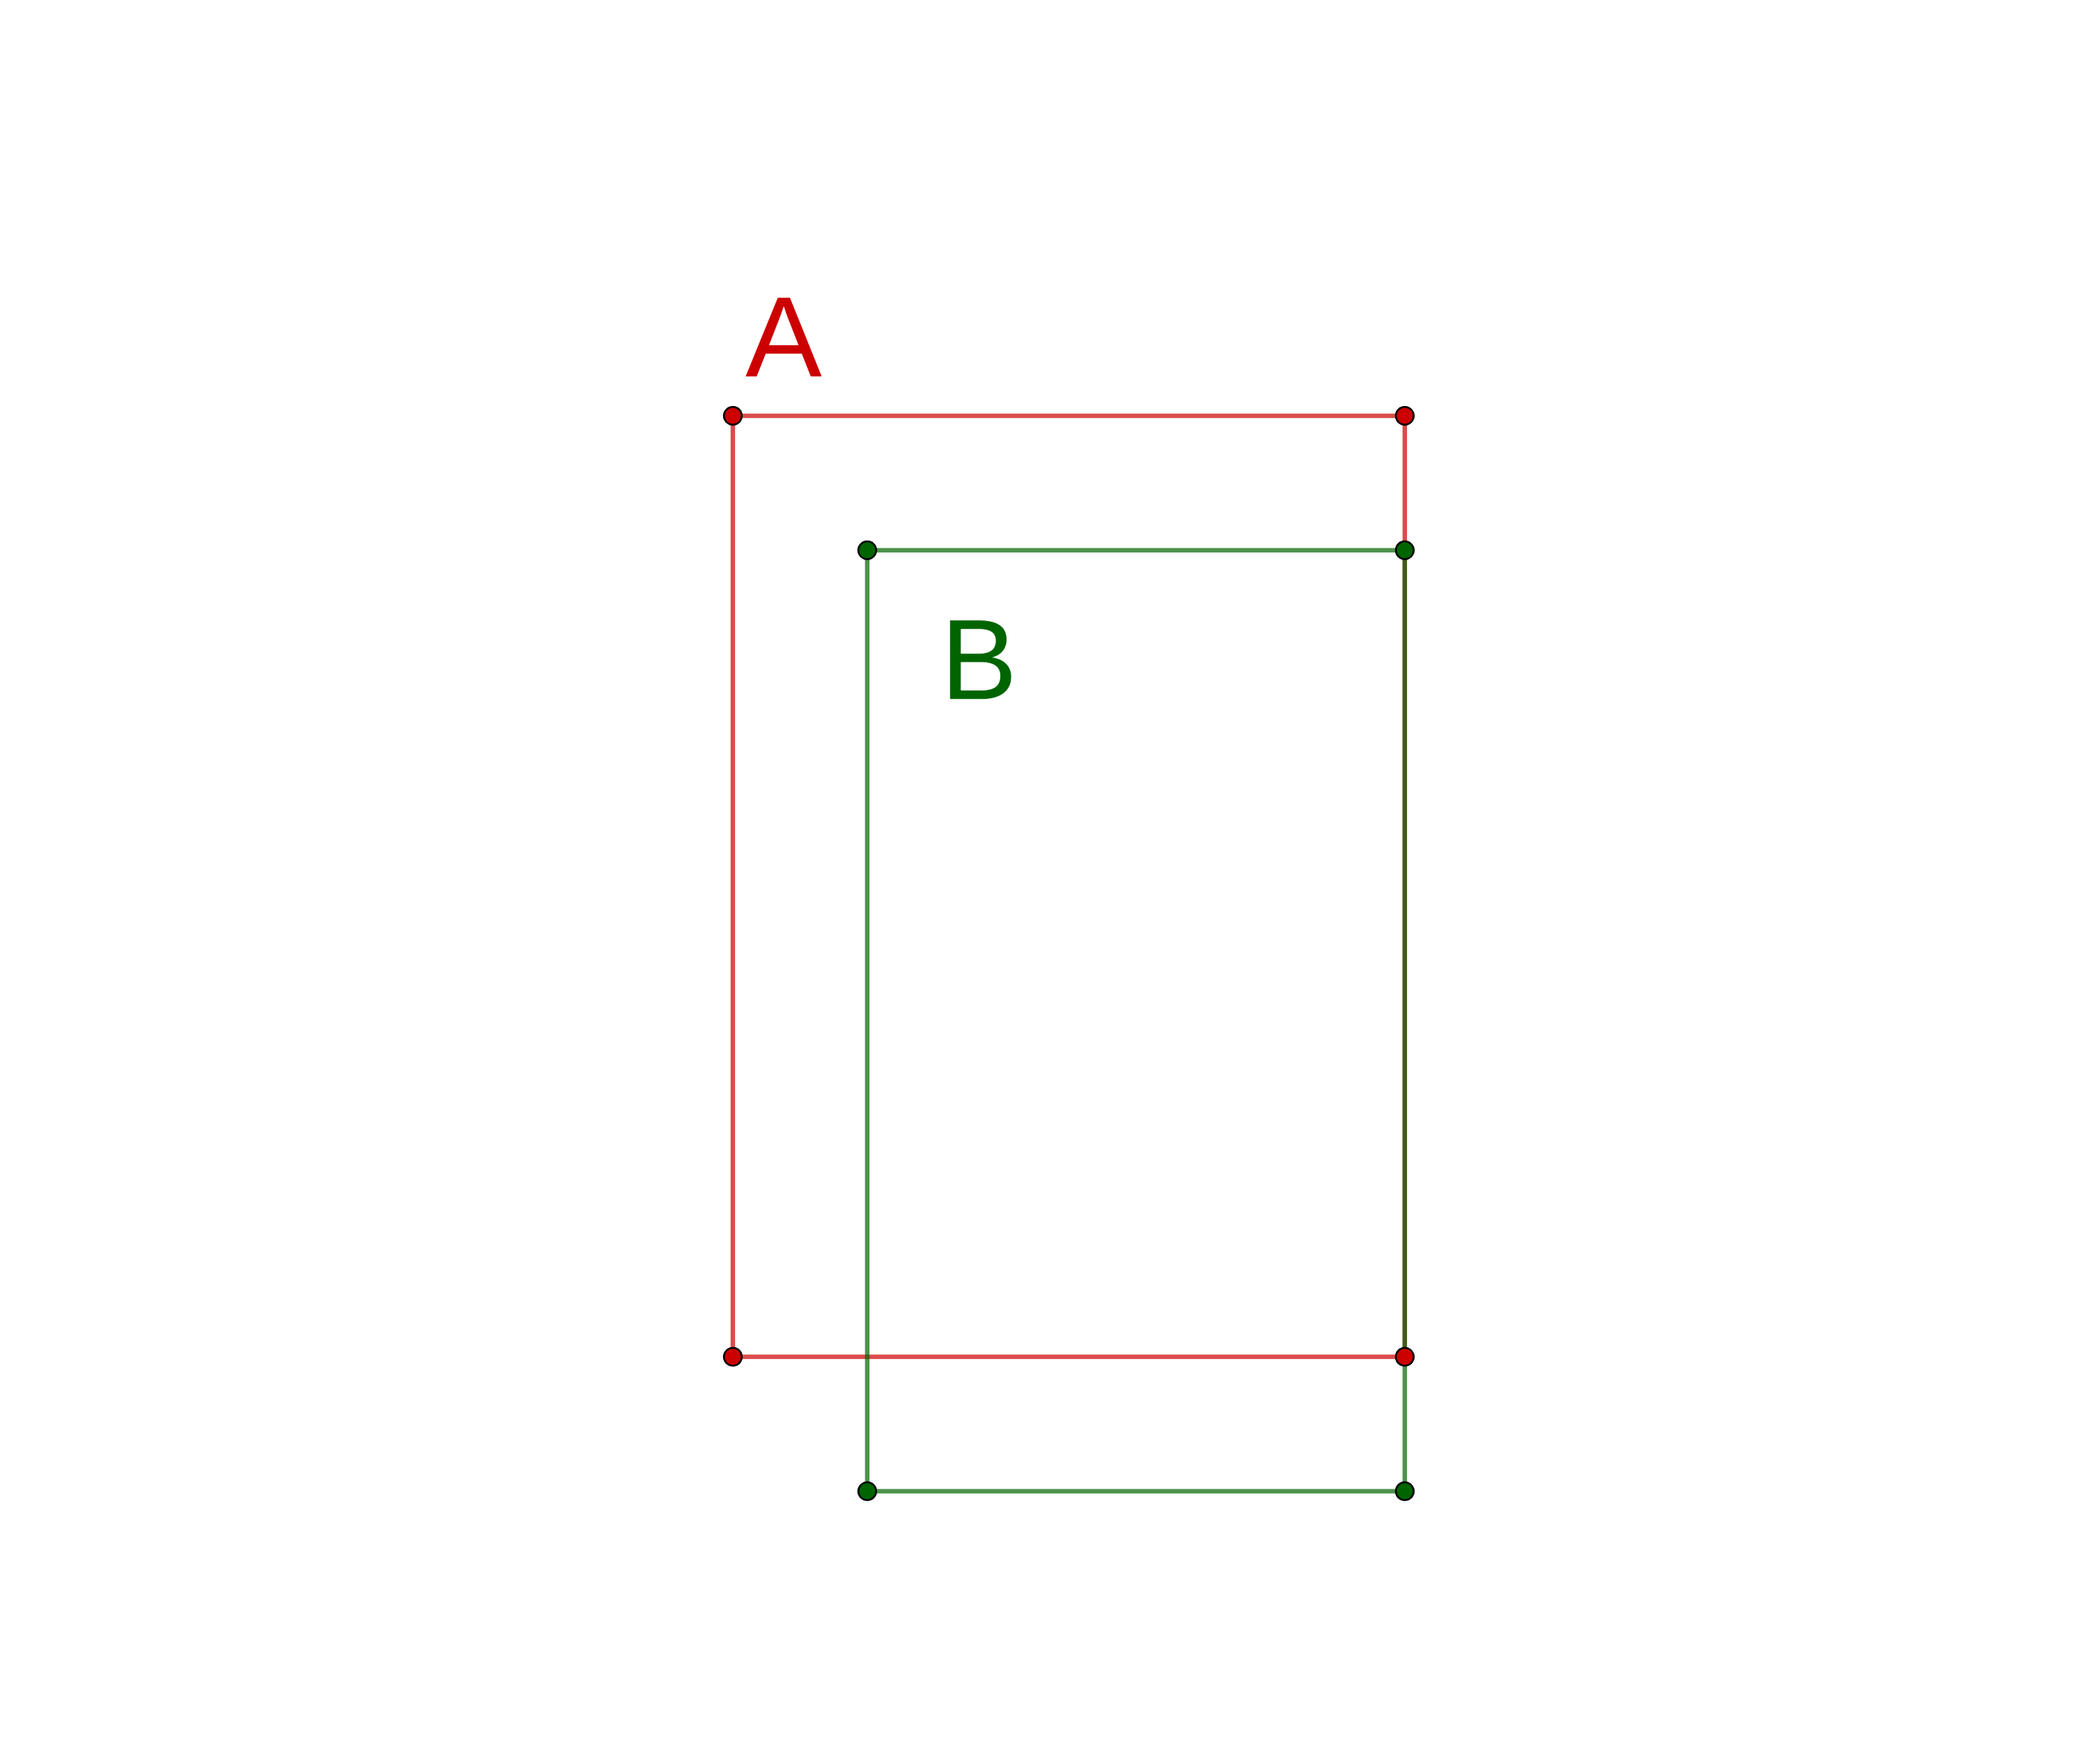
\includegraphics[scale = 0.4]{geogebra-export7.png}
        \caption*{Σχήμα 4}
    \end{figure}
    Για να αντιμετωπίσουμε αυτό το πρόβλημα βάζουμε ένα επιπλέον πεδιό-\textlatin{flag} σε κάθε κόμβο του δέντρου, που θα αντιστοιχεί στο \textlatin{rectangle} $q$ του συγκεκριμένου κόμβου και θα μας πληροφορεί για το αν 
    το $q$ έχει χρησιμοποιήθει για αναζήτηση τρίων πλευρών. Στην κατασκευή του δέντρου το \textlatin{flag} θα είναι \textlatin{FALSE}  για όλα τα $q$ και θα γίνεται \textlatin{TRUE} στην 
    επανεισαγωγή του $q$. Ο ψευδοκώδικας είναι ο παρακάτω:
    \textlatin{
\begin{algorithm}[H]
    \caption*{\textlatin{\bf Algorithm to find intersecting rectangles pairs}}
    \begin{algorithmic}
    \Function{find\_intersecting\_rectangles}{SET OF RECTANGLES}
    \For {$R$ in SET OF RECTANGLES} \Comment{Construction of the tree in $O(n \log n)$}
        \State PST.insert($R,FLAG = FALSE$)
    \EndFor 
    \For {$R$ in SET OF RECTANGLES} \Comment{Three side search for $R$}
        \State PST.remove($R$)
        \State SEARCH3S($R,PST$)
        \State PST.insert($R,FLAG = TRUE$)
    \EndFor
    \EndFunction
    \Function{Search3s}{$R,t$}
    \If{$t$ is None OR $t.q.y_2 < R.y_1$ }
        \State return
    \EndIf
    \If{$R.x_1 < t.x_{2p}$ }
        \State SEARCH3S($R,t.left$)
    \EndIf
    \If{$R.x_1 \leq t.q.x_2 \leq R.x_2$ AND $t.q.y_2 \geq R.y_1$ AND $t.q.y_1 \leq R.y_2$ }
        \State \If {NOT($R.x_2 = t.q.x_2$  AND $FLAG = TRUE$ )}
        \State report($R,t.q$) \Comment{Report intersection pair $(R,t.q)$}
        \State\EndIf
    \EndIf
    \If{$R.x_2 > t.x_{2p}$ }
    \State SEARCH3S($R,t.right$)
\EndIf
    \EndFunction
    \end{algorithmic}
    \end{algorithm}
}
Το συνολικό κόστος του αλγορίθμου θα είναι το κόστος κατασκευής του δέντρου + το συνολικό κόστος αναζήτησης 
$$O(n \log n) + O(n \log n + k) = O(n \log n + k)$$
\rule{\textwidth}{.5pt}
\section*{Άσκηση 2}
Η σχέση θα αποδειχθεί μέσω επαγωγής.
\begin{itemize}
    \item για $d=1$  $$S(1,n) = \Theta(n)= \Theta(n\log ^{d-1}n)$$
    \item για $d=2$  $$S(2,n) =2S(2,n/2) +S(1,n)=2S(2,n/2) + \Theta(n) $$
        Aπο \textlatin{master theorem} προκύπτει οτι $S(2,n) = \Theta(n\log n)=\Theta(n\log ^{d-1}n)$
    \item Εστω οτι ισχύει για $d=k$ δηλαδή $S(k,n) =\Theta(n\log ^{k-1}n)$\\
        Tότε αρκει να δείξουμε οτι για $d=k+1$ ισχύει $S(k+1,n) =\Theta(n\log ^{k}n)$:
        $$S(k+1,n) =2S(k+1,n/2) +S(k,n)=2S(k+1,n/2) + \Theta(n\log ^{k-1}n) $$
        Aπο \textlatin{master theorem} προκύπτει οτι $\gamma = \log_2 2 = 1$\\
        Αρα πρόκειται για την δεύτερη περίπτωση του \textlatin{master theorem}, όπου $f(n) =\Theta(n\log ^{k-1}n) = \Theta(n^\gamma\log ^{k-1}n)$ με $k-1>-1$\\
        Συνεπώς $S(k+1,n) =\Theta(n\log ^{k}n) $
\end{itemize}
\rule{\textwidth}{.5pt}
\section*{Άσκηση 3}
{\bf (\textlatin{a}) Υπολογισμός κόστους αναζήτησης για αναζήτηση \textlatin{rectangular range query} σε \textlatin{k-d-tree}}:\\

To πρόβλημα αναζήτησης \textlatin{rectangular range query} ανάγεται στο να εντοπίσουμε όλες τις περιοχές, στις οποίες χωρίζει τον χώρο το \textlatin{k-d-tree}, οι οποίες τέμνονται απο τα σύνορα του \textlatin{query}.  
Αυτό διότι, οτάν εντοπιστόυν οι περιοχές που τέμνουνε τα σύνορα του \textlatin{query}, τότε τα εσωτερικά σημεία του \textlatin{query} (συμπεριλαμβανομένων και των σημείων που βρίσκονται σε περιοχές που περικλείονται απο το \textlatin{query}) θα ανακτηθούν σε χρόνο $O(k)$ \\
Για τον εντοπισμό των περιοχών στα σύνορα του \textlatin{query} για δύο διαστάσεις ($d=2$) εργαζόμαστε ώς εξής:\\
Θα υπολογίσουμε την αναδρομική σχέση για τις περιοχές που τέμνονται απο μια κέθετη πλευρά του τετραγωνικου \textlatin{query} (για τις υπόλοιπες τρείς πλευρές η διαδικασία θα είναι ακριβώς η ίδια).
Oτάν κάνουμε κάθετο διαχωρισμό του χώρου στο πρώτο επίπεδο (δύο παιδιά τών $\frac{n}{2}$ στοιχείων) του δέντρου τότε η κάθετη γραμμή $l$ θά τμήσει μόνο ένα απο τα δύο παιδιά ( A και B όπως φαίνεται στο παρακάτω σχήμα).
\begin{figure}[H]
    \centering
    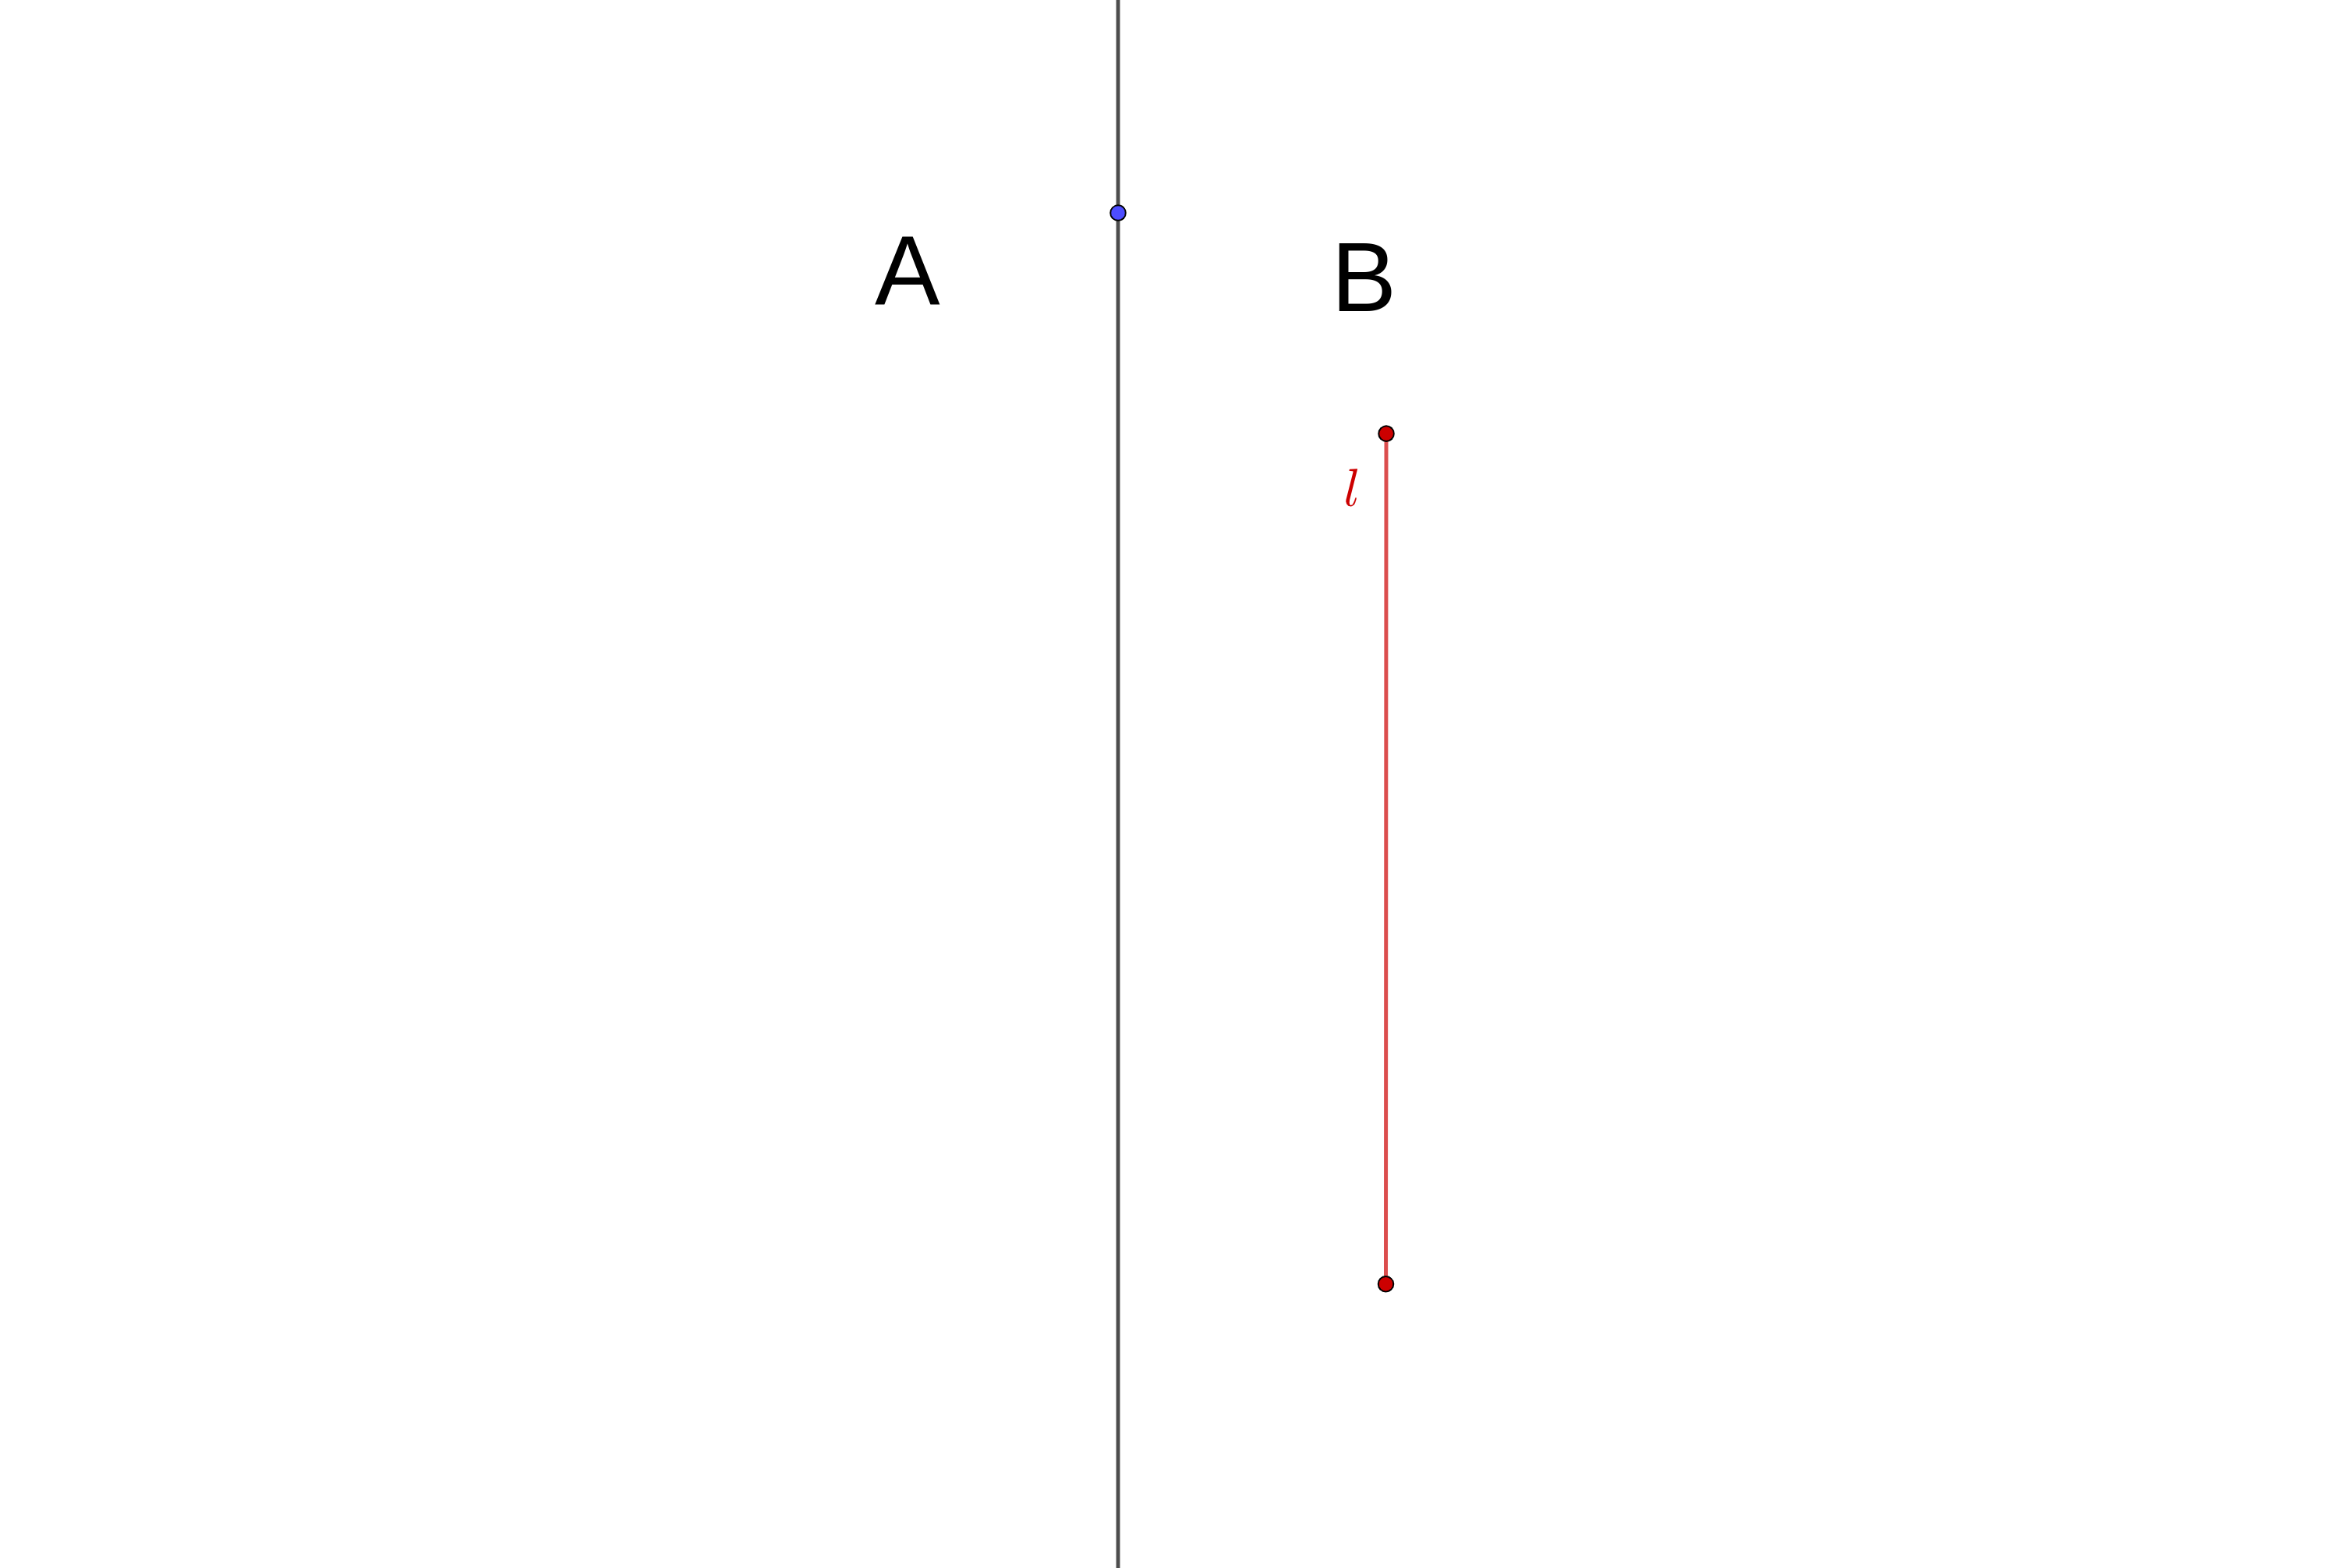
\includegraphics[scale = 0.1]{geogebra-export1.png}
\end{figure}

Αντίθετα,όταν γίνει ο οριζόντιος διαχωρισμός του χώρου στό δεύτερο επίπεδο(τέσσερα παιδιά τών $\frac{n}{4}$ στοιχείων), τότε η γράμμη $l$ θα τμήσει (στην χειρότερη περίπτωση) και τα δύο παιδιά του παιδιού B που ήδη έτεμνε απο πρίν, ενώ δεν θα τμήσει κανένα παιδι του παιδιού A.
\begin{figure}[H]
    \centering
    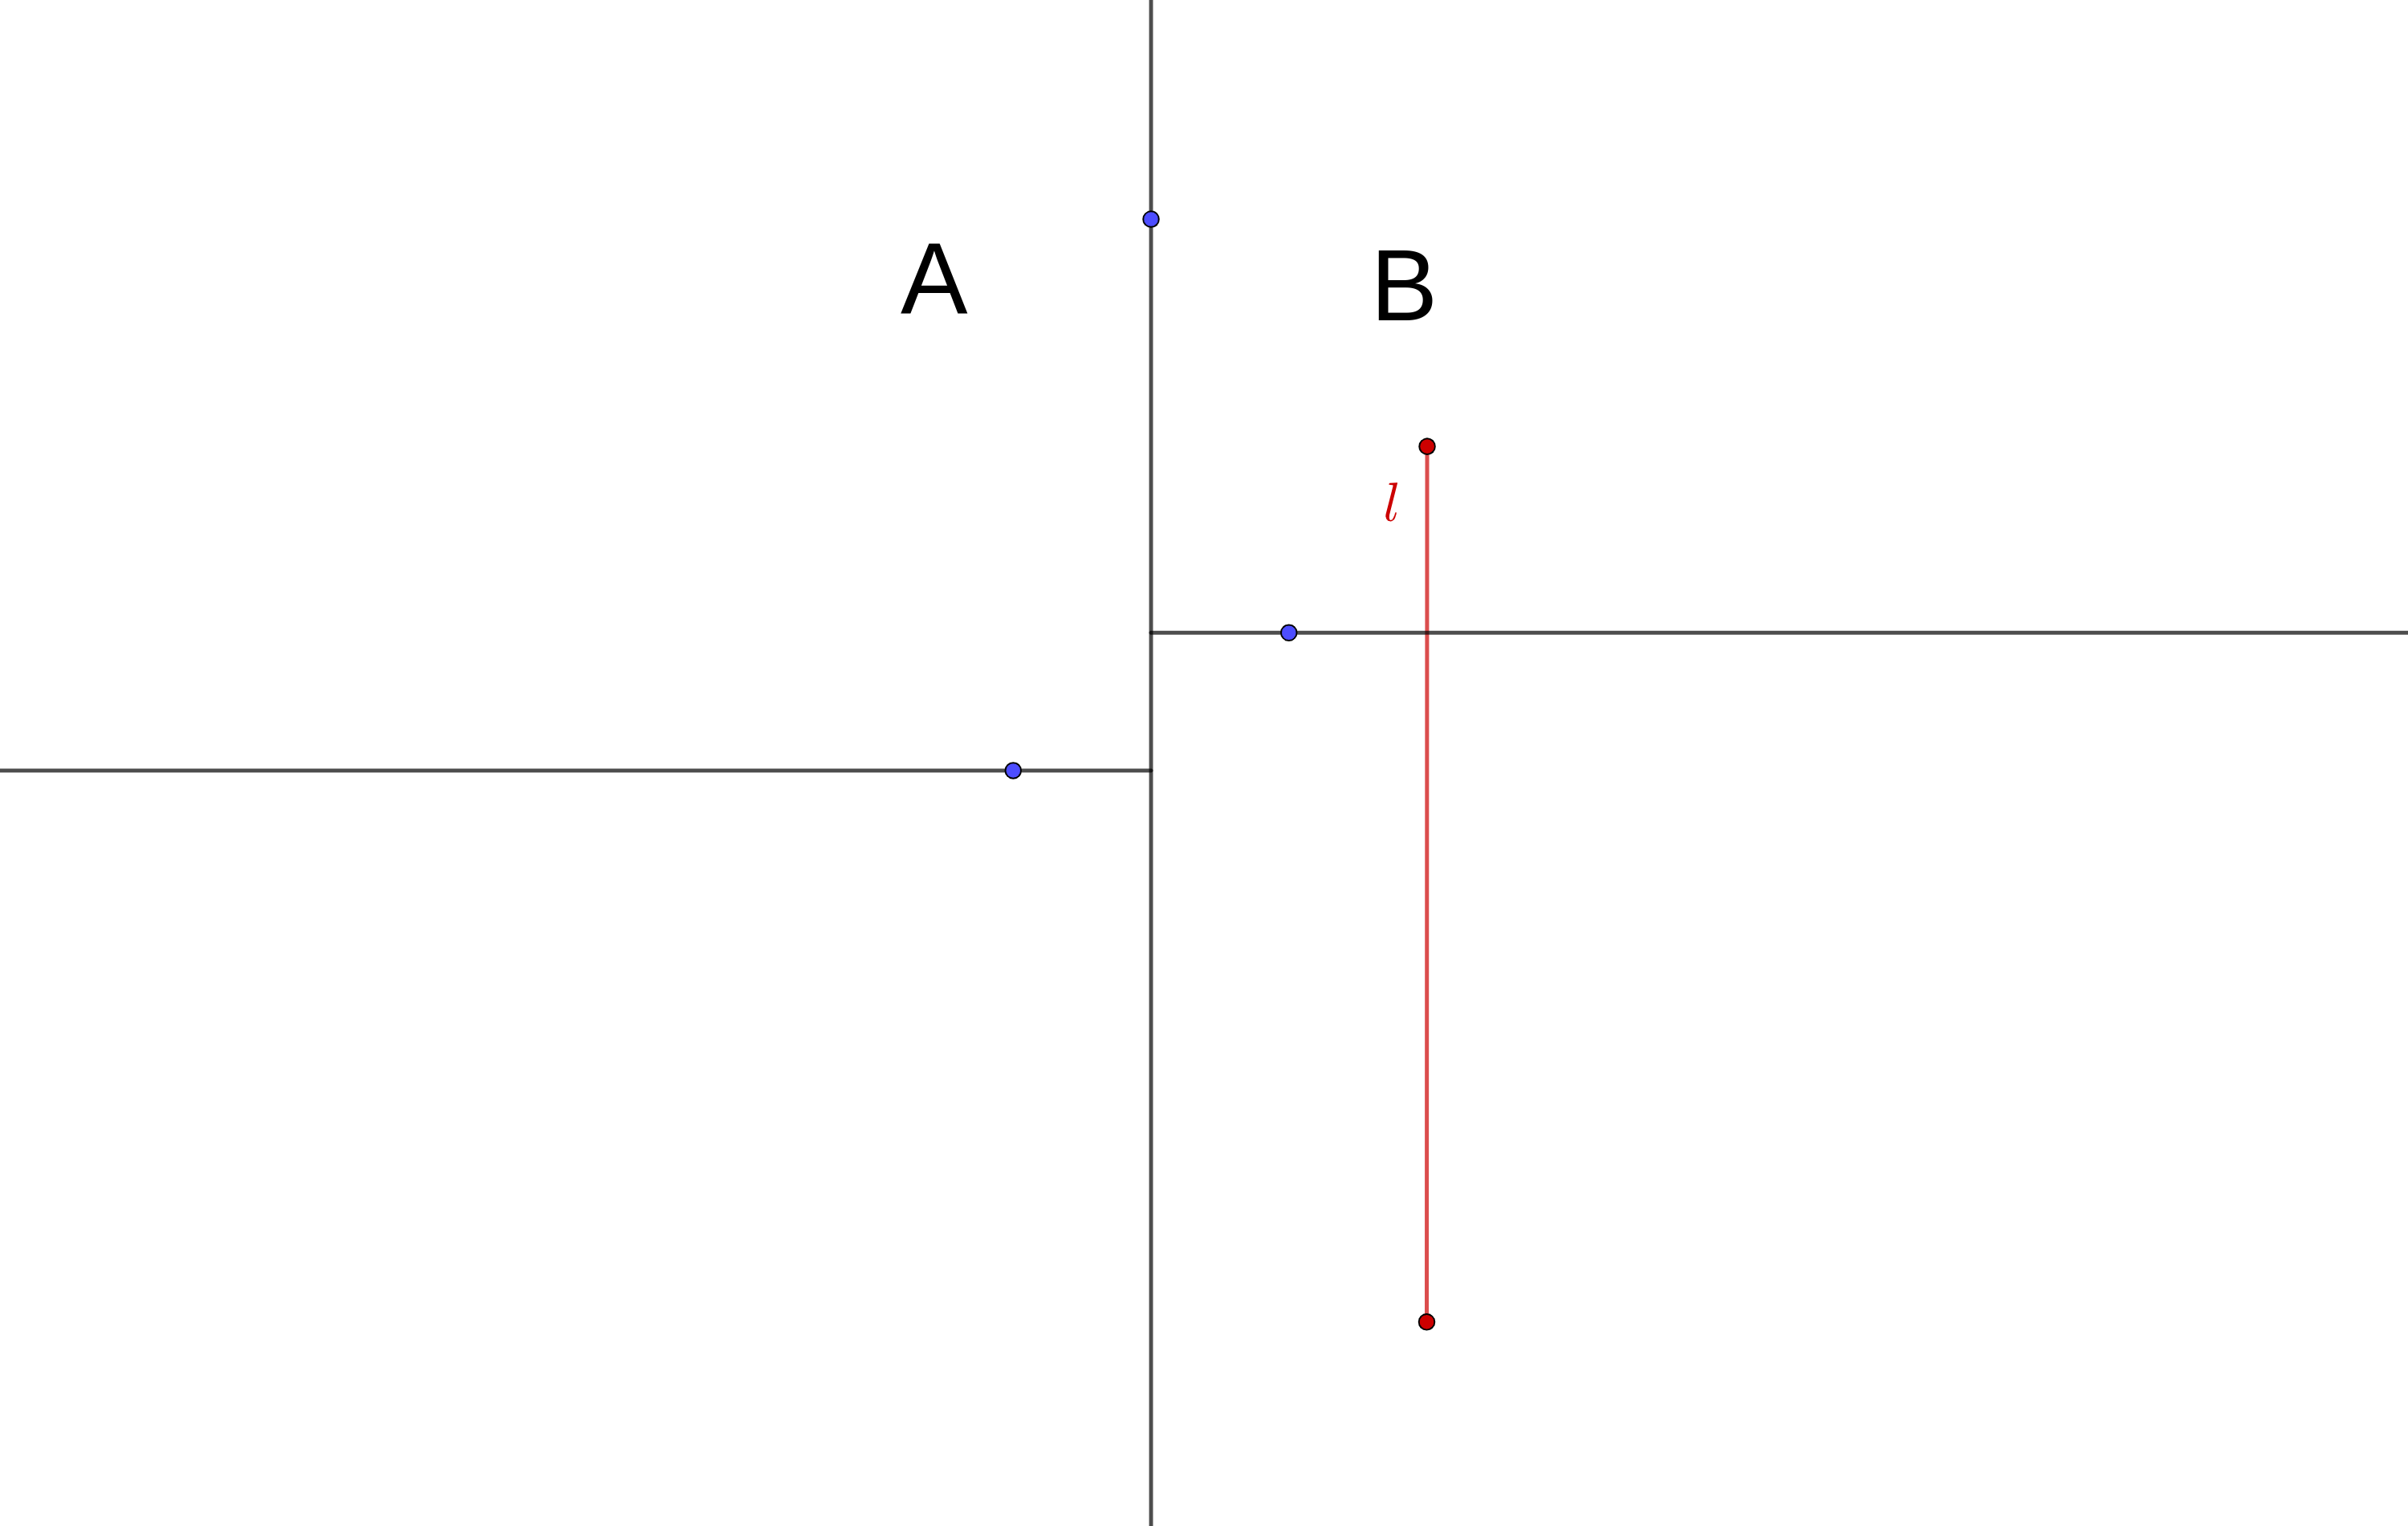
\includegraphics[scale = 0.1]{geogebra-export2.png}
\end{figure}
Άρα η αναδρομή μέχρι το δεύτερο επίπεδο θα είναι
$$Q(n) = 2 + 2Q(\frac{n}{4})$$
Απο το δεύτερο επίπεδο και έπειτα ο οριζόντιος και κάθετος διαχωρισμός εναλλάσσονται κυκλικά, άρα η παραπάνω ανδρομή θα είναι και η τελική αναδρομή του αλγορίθμου για $d=2$.\\
Γενικεύοντας στις $d$ διαστάσεις μπορούμε να πούμε οτι για κάθε διαχωρίσμο σε διάσταση παράλληλη στη πλευρά του \textlatin{query} που μελετάμε, το πλήθος των περιοχών που θα τέμνονταi απο αυτήν την πλευρα δεν θα αλλάζει. Αντίθετα,
με διαχωρισμό σε οποιαδήποτε άλλη διάσταση, το πλήθος τών περιοχών που τέμνουνται απο αυτην την πλευρα θα διπλασιάζεται. Άρα κατεβαίνοντας $d$ επίπεδα στο δέντρο, το πλήθος των περιοχών που θα τέμνονται απο 
την πλευρά του \textlatin{query} θα είναι $2^{d-1}$ και κατά συνέπεια η αναδρομή θα είναι 
$$Q(n) = 2^{d-1} + 2^{d-1}Q(\frac{n}{2^d})$$
εφαρμόζοντας \textlatin{master theorem} έχουμε:

$$\gamma = \frac{\log2^{d-1}}{\log2^d} = \frac{d-1}{d}$$
$$\rightarrow n^{\frac{d-1}{d}}>2^{d-1}$$
Aρα $$Q(n) = O(n^{\frac{d-1}{d}}) = O(n^{1-\frac{1}{d}}) $$ 
Σε συνδιασμό με τον χρόνο $O(k)$ που χρειαζόμαστε για την ανάκτηση των $k$ εσωτερικών στοιχείων, η τελική πολυπλοκότητα αναζήτησης θα είναι $Ο(n^{1-\frac{1}{d}}+k)$ \\ \\
{\bf (\textlatin{b}) Υπολογισμός κόστους κατασκευής  \textlatin{k-d-tree}}:\\
Για την κατασκευή του δέντρου, υπολογίζουμε την \textlatin{median} των $n$ σημειών σε χρόνο $O(n)$ και χωρίζουμε τον χώρο στα σε δυο υποχωρους με $\frac{n}{2}$ σημεία βάσει του \textlatin{median}. Επαναλαμβάνουμε την διαδικασία για τον κάθε υποχώρο. Συνεπώς η τελική αναδρομή θα είναι 
$$T(n) = 2T(\frac{n}{2}) + O(n)$$
Aρα απο \textlatin{master theorem} θα προκύψει οτι το κόστος κατασκευης θα είναι $Ο(n\log n)$\\
\rule{\textwidth}{.5pt}
\section*{Άσκηση 4}
Σε ένα απλό \textlatin{range tree} ο χρόνος αναζήτησης ενός \textlatin{range query} είναι $Ο(\log^d n +k)$, συνεπώς στην δική μας παραλλαγή θέλουμε να εξαλήψουμε τον όρο $O(k)$. O όρος $O(k)$
προκύπτει απο τις διαδοχικές αναφορές των σημείων που εντοπίζουμε εντός του \textlatin{range query}, όταν έχουμε φτάσει στο \textlatin{1-dimensional range tree}. Για παράδειγμα, έστω οτι έχουμε το 
\textlatin{d-dimensional range tree} στο οποίο τα κλειδιά βρίσκονται στα φύλλα και σε έναν εσωτερικό κόμβο $i$ αποθηκεύουμε to \textlatin{range} $\rho_i$ και την \textlatin{median} τιμή $z_i$ του υποδέντρου με ρίζα τον κόμβο $i$. 
Όταν κάνουμε ένα ερώτημα $\bf (a,b)$ στο δέντρο $\mathcal{R}_d$, τότε όταν φτάνουμε σε έναν \textlatin{nested} κόμβο $i$ όπου $\rho_i \subseteq (a_d,b_d)$ σύνεχίζουμε ρωτώντας το δέντρο $\mathcal{R}_{d-1}$. Οταν φτάσουμε σε \textlatin{nested} κόμβο του  $\mathcal{R}_{1}$ τότε κάνουμε διαδοχικά \textlatin{report} 
όλα του τα κλειδιά σε χρόνο $O(k)$, όπως ακριβώς θα κάναμε σε ένα απλό \textlatin{binary search tree}. Στην δική μας παραλλαγή όμως, μας ενδιαφέρει μόνο το πλήθος τών κλειδιών εντός του \textlatin{range} και οχι να τα προσδιορίσουμε ένα ένα. Άρα μπορουμε να αποφύγουμε την διαδικασία τών διαδοχικών \textlatin{reports} προσθέτοντας απλά μια μεταβλητή 
$c_i$ σε κάθε κόμβο $i$ η οποία μας πληροφορεί για το πλήθος τών κλειδιών που βρίσκονται στο υποδέντρο με ρίζα το $i$. Ετσί όταν φτάσουμε σε \textlatin{nested} κόμβο $i$ του   $\mathcal{R}_{1}$ άπλα κοιτάμε την μεταβλητή $c_i$ και επιστρέφουμε χώρις να κάνουμε \textlatin{report} τα κλειδία.
Η  αναζήτηση αυτή θα τερματίσει σε χρόνο $Ο(\log^d n)$. \\

Η κατασκευή αυτού του δέντρου θα είναι ακριβώς ίδια με του απλόύ \textlatin{range tree} με την προσθήκη του υπολογισμού της μεταβλητής $c_i$ το οποίο θέλει χρόνο $O(n)$
Αναλυτικότερα για το κόστος κατασκευής $T(n)$ έχουμε:
\begin{itemize}
    \item Ρίζα: $\rho_0 = (-\infty,\infty)$\\
        $U_0 = U$\\
        $z_0 = \textnormal{\textlatin{median}}\{x_d|x\in U_0\} \;\;\;\rightarrow\;\;\;O(n)$\\
        $ c_0 = |U_0|\;(\textnormal{το πλήθος τών }x\in U_0 )\;\;\;\rightarrow\;\;\;O(n)$\\ 
    \item Παιδιά της ρίζας :\\
    $\rho_1 = (-\infty,z_0)$ kai $\rho_2 = (z_0,\infty)$\\
    και αντίστοιχα $U_1,U_2$\\
    $U_1 = \{x\in U_0|x_d \in (-\infty, z_0]\}  \;\;\;\rightarrow\;\;\;T(n/2)$\\
    $U_2 = \{x\in U_0|x_d \in (z_0,\infty)\}  \;\;\;\rightarrow\;\;\;T(n/2)$\\
    \item Συνεχίζουμε αναδρομικά ώσπου $|U_i|=1$
    \item Σε κάθε εσωτερικό κόμβο $i$ συνδέουμε του δέντρο $\mathcal{R}_{d-1(U_i)}$
    \item Τα κλειδιά αποθηκεύοντα στα φύλλα
\end{itemize}

Αρα το τελικό κόστος κατασκευής θα προκύψει απο την αναδρομή 
$$T(n) = 2T(n/2) + 2O(n) =2T(n/2) + O(n) $$
το απο \textlatin{master theorem} δίνει $T(n) = O(n\log n)$\\
\rule{\textwidth}{.5pt}
\end{document}
